\chapter{Abbildungen}

\section{Graphen Temperatur und Luftfeuchtigkeit}
\label{Anhang_Abbildung_Temperaturverlauf}
\begin{figure}[!h] 
  \centering
     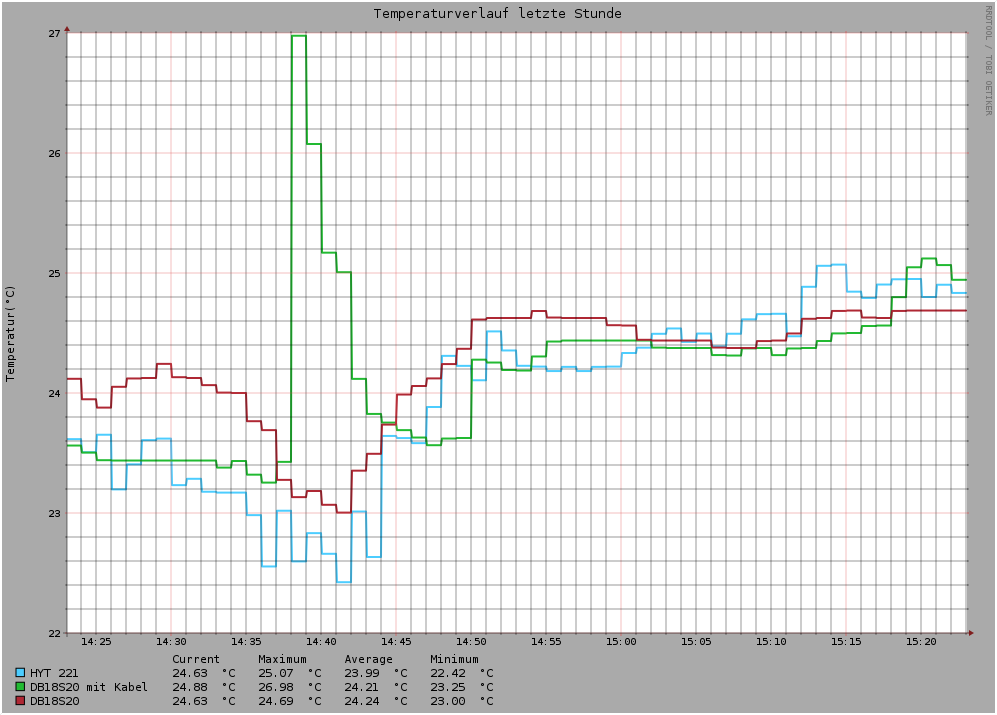
\includegraphics[scale=.3]{BilderAllgemein/Bilder/TemperaturStunde.png}
  \caption{Temperaturverlauf der letzten Stunde}
\end{figure}

\begin{figure}[!h] 
  \centering
     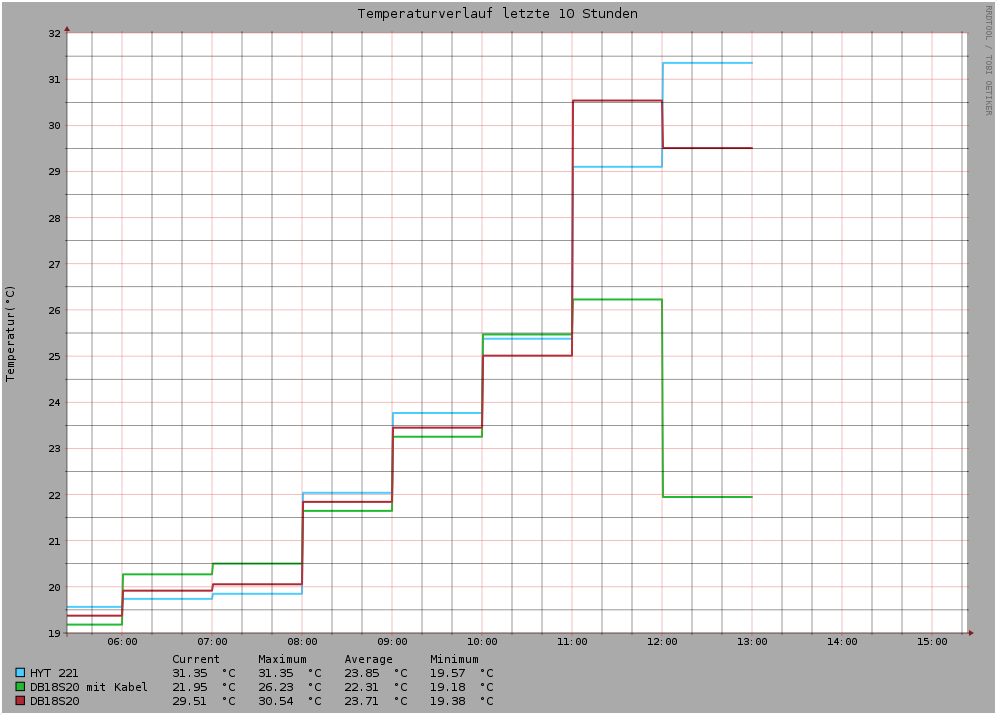
\includegraphics[scale=.3]{BilderAllgemein/Bilder/TemperaturTag.png}
  \caption{Temperaturverlauf der letzten 10 Stunden}
\end{figure}

\begin{figure}[!h] 
  \centering
     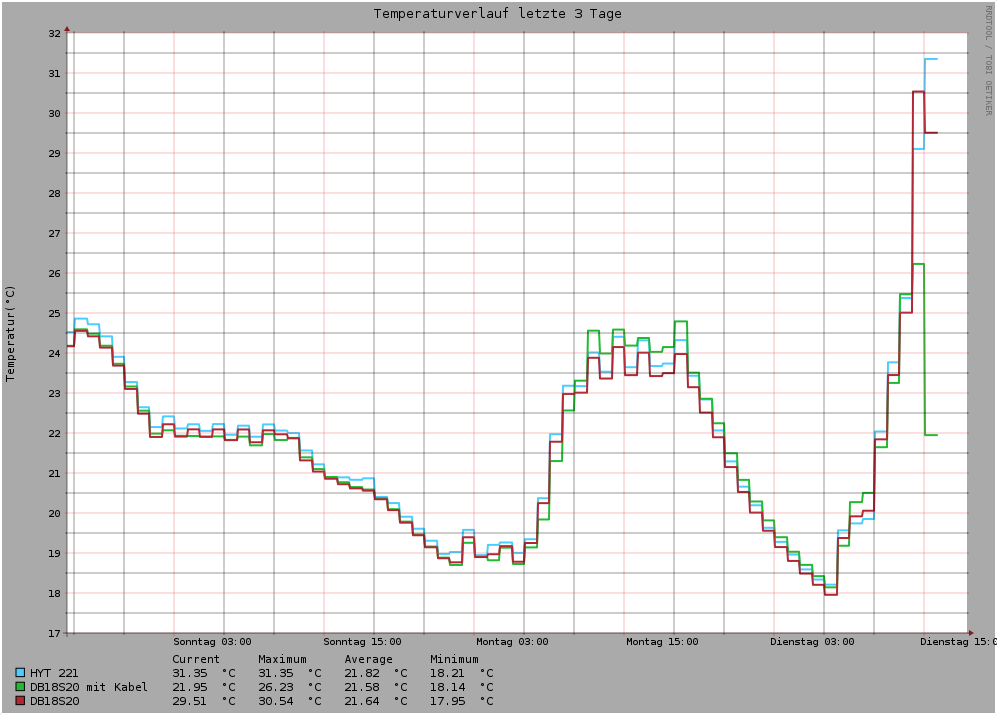
\includegraphics[scale=.3]{BilderAllgemein/Bilder/Temperatur3Tage.png}
  \caption{Temperaturverlauf der letzten 3 Tage}
\end{figure}

\begin{figure}[!h] 
  \centering
     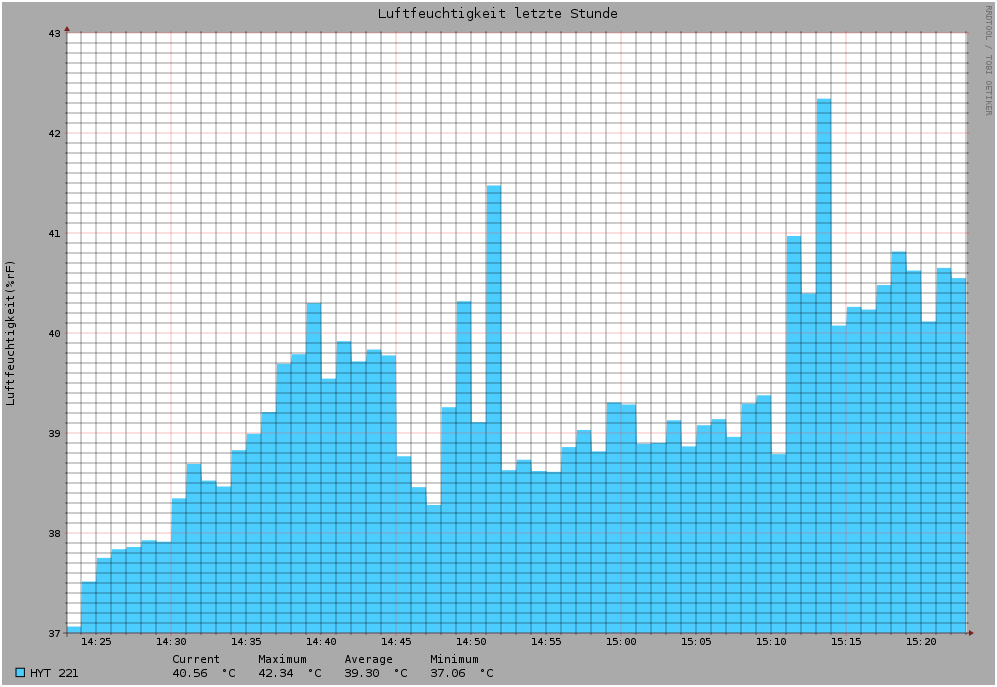
\includegraphics[scale=.3]{BilderAllgemein/Bilder/FeuchtigkeitStunde.png}
  \caption{Luftfeuchtigkeit der letzten Stunde}
\end{figure}

\begin{figure}[!h] 
  \centering
     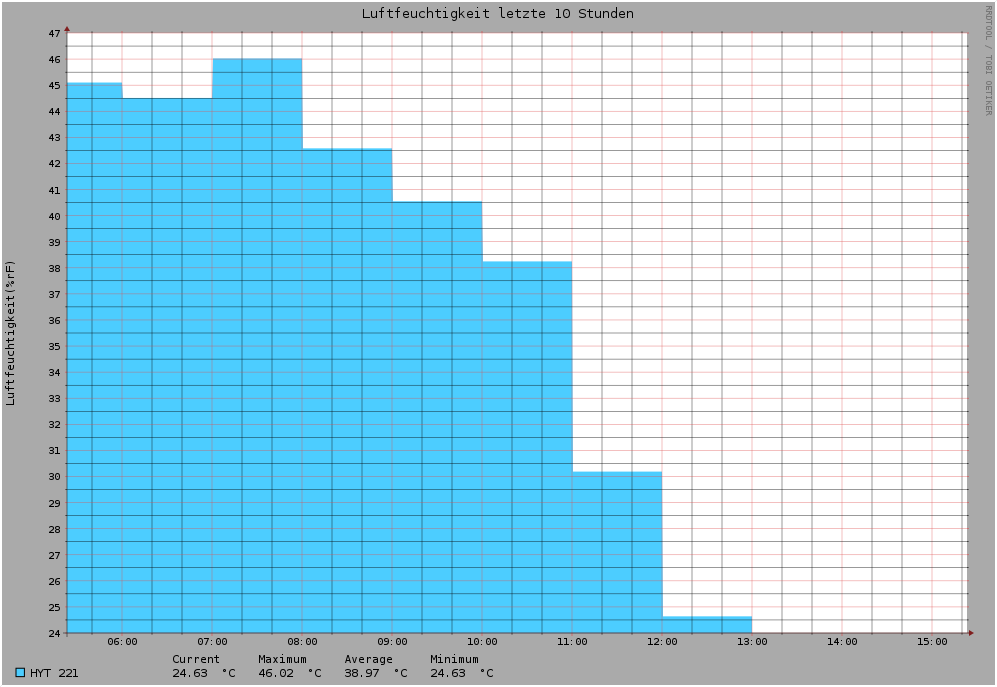
\includegraphics[scale=.3]{BilderAllgemein/Bilder/FeuchtigkeitTag.png}
  \caption{Luftfeuchtigkeit der letzten 10 Stunden}
\end{figure}

\begin{figure}[!h] 
  \centering
     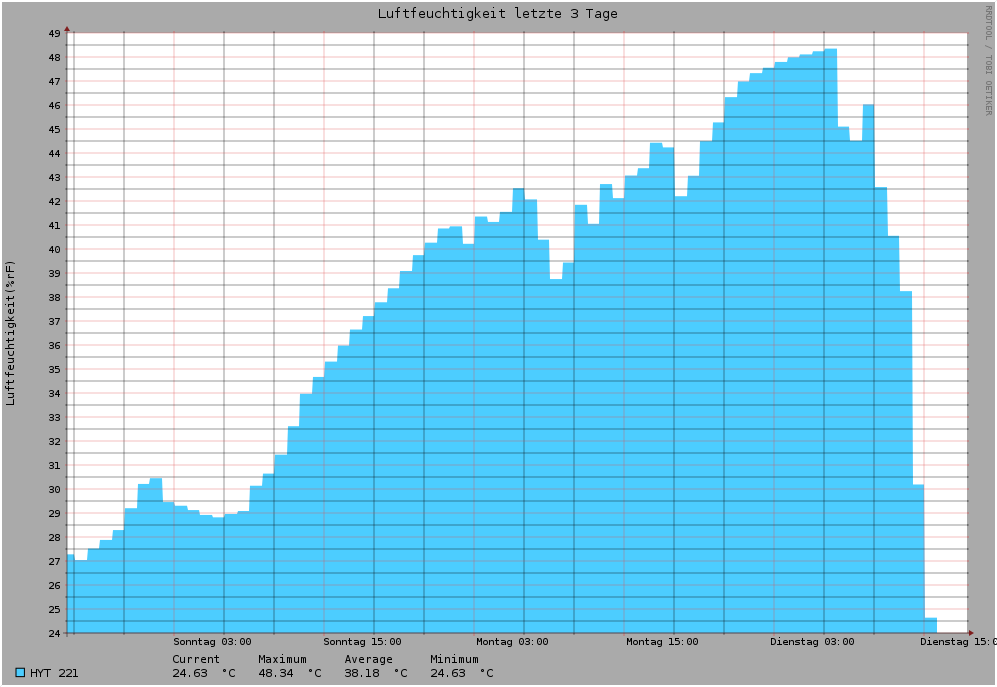
\includegraphics[scale=.3]{BilderAllgemein/Bilder/Feuchtigkeit3Tage.png}
  \caption{Luftfeuchtigkeit der letzten 3 Tage}
\end{figure}